% Author: Dr. Matthias Jung, DL9MJ
% Year: 2020
\documentclass[convert = false, border=5pt]{standalone}
\usepackage{fontspec}
\setmainfont{Roboto}
\usepackage[siunitx, straightvoltages]{circuitikzgit}
\usepackage{tikz}


\usepackage{pgfplots}
\usetikzlibrary{decorations.pathmorphing}
\pgfplotsset{width=7cm,compat=1.8}
\pgfplotsset{
    colormap/outside/.style={
        colormap=
            {outside}{
            rgb255(0cm)=(255,255,255);
            rgb255(1cm)=(255,255,255);
            }
    },
    colormap/outside,
    colormap/inside/.style={
        colormap={inside}{
            rgb255(0cm)=(255,255,255);
            rgb255(1cm)=(255,255,255);
        }
    },
    colormap/inside
}
\begin{document}
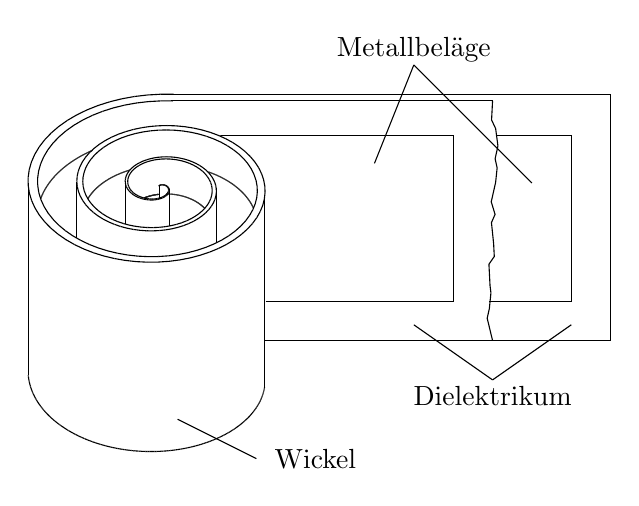
\begin{tikzpicture} [
  pencildraw/.style={
    black,
    decorate,
    decoration={random steps,segment length=5pt,amplitude=2pt}
  }
]
  %\tikzstyle{help lines}=[blue!50];
  %\draw[style=help lines] (0,0) grid (8,6);
  %
  %\definecolor{jazz}{rgb}{0.90196078431,0.90196078431,0.90196078431}
  \fill[white] (2.41,5.125) rectangle (8,2);
  \filldraw[fill=white] (2.41,4.6) rectangle (6,2.5);
  %
  \begin{axis}[
      hide axis,
      axis equal image,
      z buffer=sort,
      view={30}{40},
      width=15cm
    ]
    \addplot3 [ % 3D Spirale
      surf,
      domain=0:3*352,
      samples=200,
      y domain=0:2000,
      samples y=2,
      mesh/interior colormap name=inside,
      colormap/outside,
      shader=flat,
      variable=\t,
      point meta={cos(t)},
      faceted color=black,
    ]
    (
      {sin(t)*1.1*(t)},
      {cos(t)*1.1*t},
      {y}
    );
    \addplot3 [ % Rand oben
      surf,
      domain=0:3*352,
      samples=200,
      y domain=0:2000,
      samples y=2,
      shader=faceted,
      variable=\t,
      faceted color=black,
    ]
    ( 
      {sin(t)*1.1*(t)},
      {cos(t)*1.1*t},
      {2000}
    );
    %\addplot3 [ % Rand oben
    %  surf,
    %  domain=0:3*352,
    %  samples=200,
    %  y domain=0:2000,
    %  samples y=2,
    %  shader=faceted,
    %  variable=\t,
    %  faceted color=red,
    %  dashed
    %]
    %( 
    %  {sin(t)*1.02*(t)},
    %  {cos(t)*1.02*t},
    %  {1630}
    %);
    \addplot3 [ % Element für Metallbelag
      surf,
      domain=976:1019,
      samples=200,
      y domain=0:2000,
      samples y=2,
      shader=faceted,
      variable=\t,
      faceted color=black,
    ]
    ( 
      {sin(t)*1.02*(t)},
      {cos(t)*1.02*t},
      {1630}
    );
    \addplot3 [ % Element für Metallbelag 2
      surf,
      domain=626:670,
      samples=200,
      y domain=0:2000,
      samples y=2,
      shader=faceted,
      variable=\t,
      faceted color=black,
    ]
    ( 
      {sin(t)*1.02*(t)},
      {cos(t)*1.02*t},
      {1630}
    );
    \addplot3 [ % Element für Metallbelag 3
      surf,
      domain=723:768,
      samples=200,
      y domain=0:2000,
      samples y=2,
      shader=faceted,
      variable=\t,
      faceted color=black,
    ]
    ( 
      {sin(t)*1.02*(t)},
      {cos(t)*1.02*t},
      {1630}
    );
    \addplot3 [ % Element für Metallbelag 4
      surf,
      domain=308:330,
      samples=200,
      y domain=0:2000,
      samples y=2,
      shader=faceted,
      variable=\t,
      faceted color=black,
    ]
    ( 
      {sin(t)*1.02*(t)},
      {cos(t)*1.02*t},
      {1630}
    );
    \addplot3 [ % Element für Metallbelag 5
      surf,
      domain=340:397,
      samples=200,
      y domain=0:2000,
      samples y=2,
      shader=faceted,
      variable=\t,
      faceted color=black,
    ]
    ( 
      {sin(t)*1.02*(t)},
      {cos(t)*1.02*t},
      {1630}
    );
    \addplot3 [ % Rand oben
      surf,
      domain=0:3*352,
      samples=200,
      y domain=0:2000,
      samples y=2,
      shader=faceted,
      variable=\t,
      faceted color=black,
    ]
    ( 
      {sin(t)*1.02*(t)},
      {cos(t)*1.02*t},
      {2000}
    );
    \addplot3 [ % Unten
      surf,
      domain=790:3*320,
      samples=200,
      y domain=0:2000,
      samples y=2,
      shader=faceted,
      variable=\t,
      faceted color=black,
    ]
    ( 
      {sin(t)*1.1*(t)},
      {cos(t)*1.1*t},
      {0}
    );
  \end{axis}
  % Further outlines:
  \draw(0.603,1.56) -- (0.603,4);
  \draw(3.603,1.40) -- (3.603,3.8);
  %
  \draw(1.220,3.305) -- (1.220,4.010);
  \draw(2.990,3.235) -- (2.990,3.940);
  %
  \draw(1.835,3.477) -- (1.835,4.010);
  \draw(2.394,3.450) -- (2.394,3.920);
  %
  \draw(2.265,3.800) -- (2.265,3.972);
  %
  \draw(2.415,5.127) -- (8,5.127) -- (8,2) -- (3.603,2);
  \draw(2.415,5.043) -- (6.5,5.043);
  %
  \draw(6.55,4.60) -- (7.5,4.6) -- (7.5,2.5) -- (6.46,2.5);
  %
  \pgfmathsetseed{43} % Um die Form gleich zu halten
  \draw[pencildraw](6.5,5.043) -- (6.5,2); 
  %
  \draw(4.25,0.5) node[](){Wickel};
  \draw(5.5,5.7) node[](){Metallbeläge};
  \draw(6.5,1.3) node[](){Dielektrikum};
  %
  % Wickel:
  \draw(3.5,0.5) -- (2.5,1.0);
  % Metallbeläge:
  \draw(5.5,5.5) -- (5.0,4.25);
  \draw(5.5,5.5) -- (7.0,4.00);
  % Dielektrikum:
  \draw(6.5,1.5) -- (5.5,2.2);
  \draw(6.5,1.5) -- (7.5,2.2);
\end{tikzpicture}
\end{document}
